\section{Computação Clássica} 
Entende-se a importância de se compreender a origem e o desenvolvimento da computação clássica para o desenrolar da pesquisa, o que será apresentado em meio a este capítulo.

A computação clássica consiste em computadores que dependem da física clássica para operar. Estes são os computadores tradicionais que usamos em nosso dia-a-dia – seja eles Apple, Samsung, Dell ou qualquer outro –, também classificados como computadores binários, pois processam as instruções a partir de números binários, compostos apenas pelos símbolos “1” e “0”, ligado e desligado, respectivamente. Assim, julga-se importante e de larga relevância ao tema compreender essa representação numérica. 

Números binários ou números em base 2 são compostos por apenas dois dígitos, [0...1]. Dessa forma, seu funcionamento é similar ao sistema decimal, ou base 10, que são compostos por dez dígitos, [0...9]. No sistema decimal, é simples contar até nove, porém não existe um simbolo ou dígito para representar o número dez, sendo então representado por dois dígitos, “10”, sendo uma simples lógica de posicionamento. Mais uma vez, após o número “99”, é necessário utilizar da mesma regra para representar o número cem, “100”. Já em base 2, o número zero é representado pelo simbolo ``0'', e o número um por ``1''. O mesmo dilema é enfrentado ao chegar no próximo valor: dois. E então é usada a mesma lógica de posicionamento, em base dois. Desta forma, o número dois é representado por “10”, o três por “11”, quatro por “100” e assim por diante. Portanto, números binários podem se tornar longos e compostos por muitos dígitos que levam o nome de bits. \cite{6} É com base nos \label{bits}bits\footnote{A menor unidade de informação que pode ser armazenada ou transmitida na comunicação de dados.} ligados e desligados que o computador baseia a sua linguagem. Para transforma-lo em base dez é preciso avaliar o valor de cada bit de acordo com a sua posição. 

Exemplo: número binário $1011$:

\[ 1011(b) = 1*2^3 + 0*2^2 + 1*2^1 + 1*2^0\]
\[ = 8 + 0 + 2 + 1 = 11(decimal)\]

O peso de cada bit de um número binário depende da sua posição relativa ao número completo, sempre partindo da direita para a esquerda.

\begin{itemize}
  \item O peso do primeiro bit é $bit * 2^0$
  \item O peso do segundo bit é $bit * 2^1$
  \item O peso do terceiro bit é $bit * 2^2$
  \item O peso do quarto bit é $bit * 2^3$
\end{itemize}

A formúla ilustrada acima, pode ser exemplificada em uma fórmula genérica: 

\[= nth\: bit * 2^{n-1}\]

É possível notar que a regra para números binários, se repete para números em base 10.

Exemplo: número decimal $4392$:
\begin{itemize}
  \item O peso do primeiro bit é $2 * 10^0$
  \item O peso do segundo bit é $9 * 10^1$
  \item O peso do terceiro bit é $3 * 10^2$
  \item O peso do quarto bit é $4 * 10^3$
\end{itemize}
\[ 4392 = 4*10^3 + 3*10^2 + 9*10^1 + 2*10^0\]
\[= nth\: bit * 10^{n-1}\]

Essa regra se mantem verdadeira para qualquer base númerica.

\[= nth\: bit * (base)^{n-1}\]

Ao decorrer do texto serão referidos números em base 2, 10 e 16. 

\subsection{A computação clássica e sua evolução}
Alan Turing, matemático inglês, cientista da computação, lógico, criptoanalista, filósofo e biólogo teórico, publicou o artigo “On Computable Numbers with an Application to the Entscheidungs-problem” \cite{8} em 12 de novembro de 1937, esse formaria a teoria básica da computabilidade por várias décadas.

O mecanismo abstrato descrito no artigo de Turing fornece os conceitos fundamentais de computadores que outros engenheiros conceberam posteriormente. Na sua essência, uma Máquina de Turing é um dispositivo que manipula símbolos em uma tira de fita de acordo com uma tabela de regras. O cientista forneceu a formalização dos conceitos de “algoritmo” e “computação” na infância da ciência da computação. Apesar de sua simplicidade, uma Máquina de Turing pode ser adaptada para simular a lógica de qualquer algoritmo de computador e é útil para explicar as funções de uma CPU.

Apesar dos computadores clássicos serem atualmente descritos como tendo a chamada arquitetura de Von Neumann, acredita-se que o idealizador dessa arquitetura partiu dos modelos matemáticos desenvolvidos por Alan Turing, que incluia o conceito de programa armazenado, originado a partir da construção da Maquina de Turing. Conceito também encontrado no projeto EDVAC de Von Neumann \cite{9}, que possibilita o armazenamento de instruções e dados na mesma memória, permitindo a manipulação de programas como dados, que se constitui como característica definidora do computador clássico. Assim, pode-se alegar que Turing é o pai do computador já que suas publicações antecedem a arquitetura de Von Neumann, além de existirem razões para se acreditar que este último conhecia os resultados do trabalho de Alan Turing \cite{10}, que podem ter inspirado as suas criações. Outro fator que corrobora para este entendimento, é que Turing foi o primeiro a explorar a idéia de uma máquina de uso geral por meio de sua noção de máquina universal – que constitui a base do computador clássico ao possibilitar o funcionamento da CPU em conjunto com a memória RAM. Ainda tendo em vista as contribuições do matemático para a construção de uma classe importante de dispositivos de computação, o Bombe – um dispositivo eletromecânico usado pelos criptologistas britânicos para ajudar a decifrar as mensagens secretas criptografadas pela máquina alemã Enigma durante a Segunda Guerra Mundial – e posteriormente o seu design do ACE (Automatic Computing Engine), fica evidente as contribuições de Alan Turing para a invenção do computador moderno. A partir da fala de Turing abaixo, pode-se identificar o ACE como um tipo de realização física da máquina universal.

\textit{
  ``Some years ago I was researching on what might now be described as an investigation of the theoretical possibilities and limitations of digital computing machines. […] Machines such as the ACE may be regarded as practical versions of this same type of machine.'' \cite{11}
}

Por fim, conclui-se que baseado na teoria da máquina de Turing, o físico e matemático John von Neumann desenvolveu uma arquitetura que era capaz de executar as seguintes tarefas.

\vspace{1cm}
\begin{figure}[H] \centering 
  \makebox[\textwidth][c]{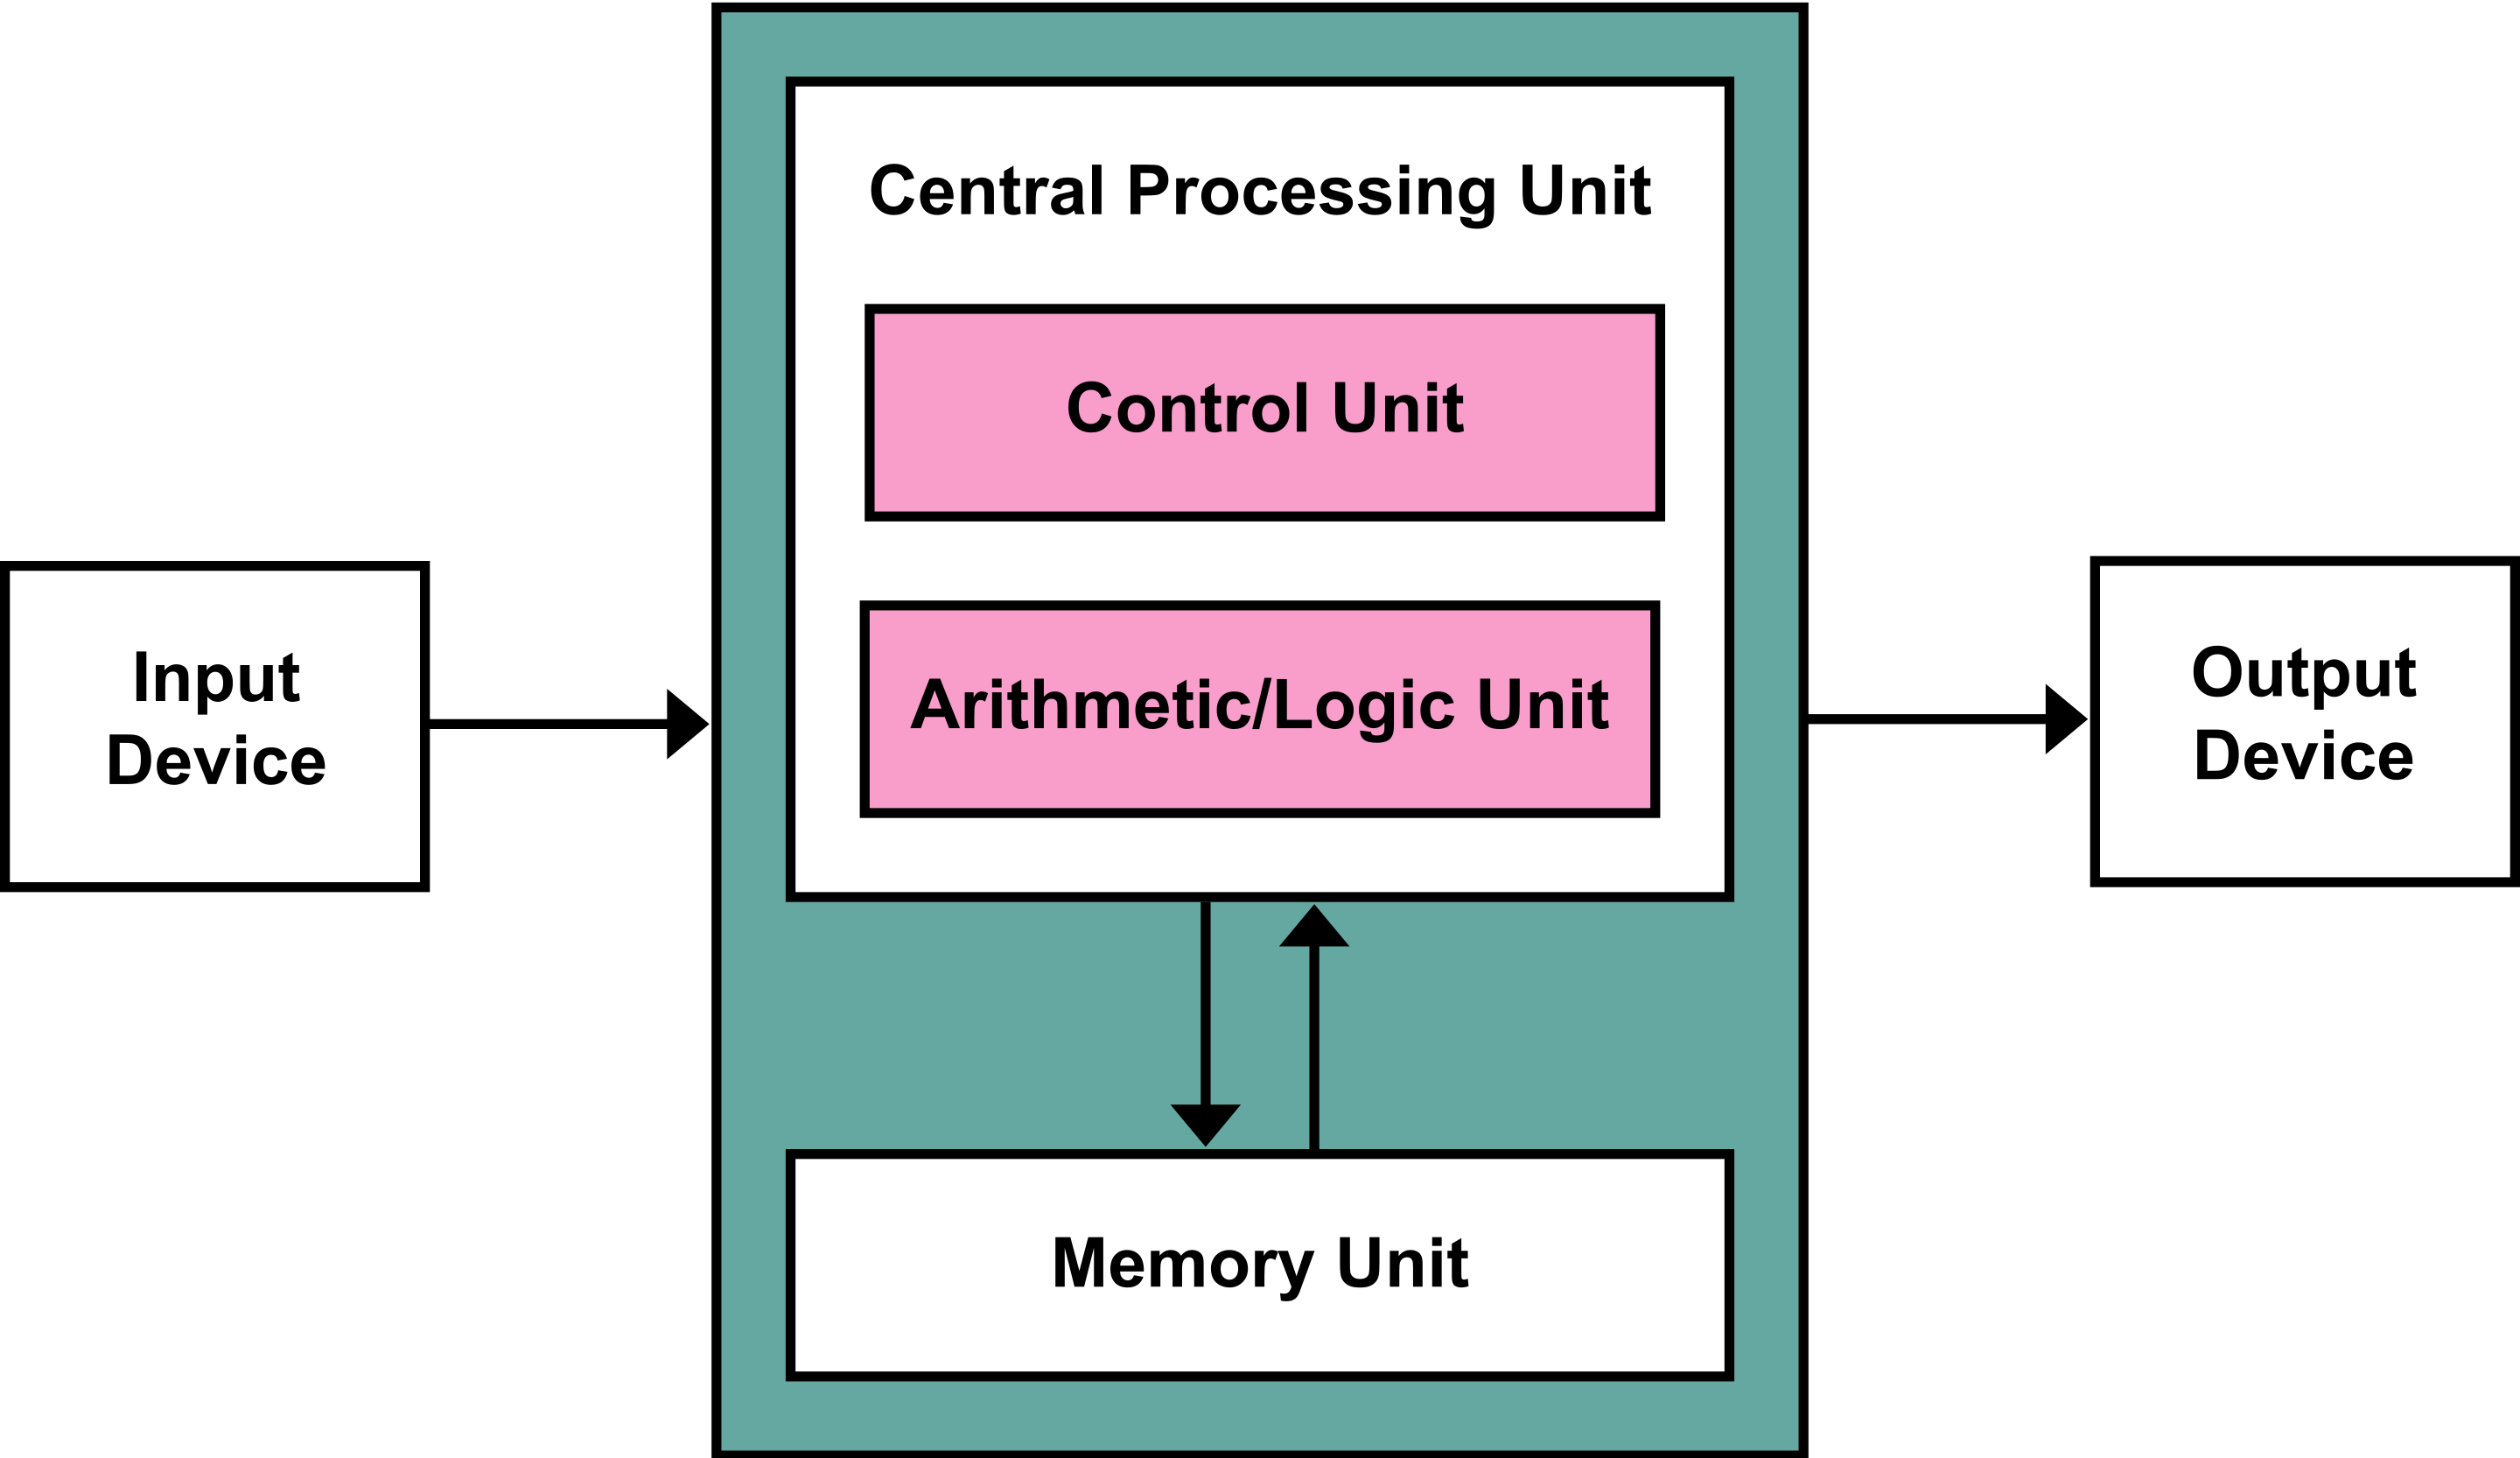
\includegraphics[width=0.8\textwidth]{von_neumann_architecture}}
  \caption{\label{fig:1} Diagrama arquitetura de Von Neumann} 
\end{figure}

Nessa arquitetura, o cabeçalho passa a ser uma CPU (Central Processing Unit), a fita se transforma em memória RAM e as operações são construidas e executadas em circuitos formados por portas lógicas  chamadas de ALU (Arithmetic/Logic Unit). \cite{12}

Atualmente, a maioria dos computadores modernos são construídos sobre a praxis da arquitetura von Neumann. A fim de simular um processador moderno de forma didática, foi elaborado o \href{https://gzsig.io/vm-24bits/}{ASM 24bits} que apresenta as principais características de um processador moderno e permite a sua programação utilizando um Assembly\footnote{Uma linguagem assembly é uma linguagem de programação de baixo nível projetada para um tipo específico de processador. Ele pode ser produzido compilando o código-fonte de uma linguagem de programação de alto nível (como C / C ++), mas também pode ser escrito do zero.} de 20 instruções, sua \href{https://github.com/gzsig/Asm/blob/master/README.md}{Documentação}. Similar à arquitetura de von Neumann esse emulador é composto por memória e CPU, essa CPU simples possui 2 registradores, eles são :

\vspace{1cm}
\begin{longtable}{ |p{3cm}||p{11cm}|  }
  \hline
  \multicolumn{2}{|c|}{Registradores} \\
  \hline
    Nome &
    Descrição\\
  \hline
    Accumulator (ACC) &Este é o registro mais usado para armazenar dados extraídos da memória. Está em diferentes números em diferentes microprocessadores.\\
  \hline
    Instruction Register (IR) &É o registro que contém a instrução que está sendo executada atualmente.\\
  \hline
\end{longtable}
\vspace{1cm}

Uma unidade lógica aritmética (ALU) é um circuito digital usado para realizar operações aritméticas e lógicas. Ele representa o bloco de construção fundamental da unidade central de processamento CPU. A ULA do ASM 24bits possui 20 instruções, sendo elas:

\vspace{1cm}
\begin{longtable}{ |p{3cm}||p{11cm}|  }
  \hline
  \multicolumn{2}{|c|}{ULA} \\
  \hline
  Mnemônico &
  Descrição\\
  \hline
  nop &
  Slot de memória vazio \\
  \hline
  jmp &
  Salto incondicional. Recebe uma variável como parâmetro e executará o código a partir da linha abaixo. \\
  \hline
  jz &
  Salta se o valor do acumulador (AC) é 0. Recebe uma variável como parâmetro e executará o código a partir da linha abaixo se o valor do AC for zero. Se o valor de AC NÃO for zero, a próxima linha será executada. \\
  \hline
  jnz &
  Pula se o valor do acumulador (AC) NÃO é 0. Recebe uma variável como parâmetro e executará o código a partir da linha abaixo se o valor do AC não for zero. Se o valor de AC for zero, a próxima linha será executada. \\
  \hline
  lv &
  Carregue uma constante diretamente no acumulador. Recebe uma constante em notação hexadecimal 0x00F2 por exemplo. \\
  \hline
  add &
  Adicione uma constante ao valor do acumulador. Recebe uma constante em notação hexadecimal 0x00FA por exemplo. \\
  \hline
  addm &
  Recebe uma variável como parâmetro e adiciona o valor da variável ao valor do acumulador. \\
  \hline
  sub &
  Subtraia uma constante do valor do acumulador. Recebe uma constante em notação hexadecimal 0x00FA por exemplo. \\
  \hline
  subm &
  Recebe uma variável como parâmetro e subtrai o valor da variável do valor do acumulador. \\
  \hline
  mul &
  Multiplique uma constante do valor do acumulador. Recebe uma constante em notação hexadecimal 0x00FA por exemplo. \\
  \hline
  mulm &
  Recebe uma variável como parâmetro e multiplica o valor da variável pelo valor do acumulador. \\
  \hline
  div &
  Divide o valor do acumulador por uma constante. Recebe uma constante em notação hexadecimal como parâmetro, 0x00FA por exemplo. \\
  \hline
  divm &
  Recebe uma variável como parâmetro e divide o valor do acumulador pelo valor da variável. \\
  \hline
  load &
  Recebe uma variável como parâmetro e carrega o valor da variável para o acumulador. \\
  \hline
  stor &
  Armazene o valor atual do acumulador em uma variável. \\
  \hline
  sc &
  Chamada de função. \\
  \hline
  rc &
  Retorno de função, irá pular para a linha abaixo da chamada de função mantendo o valor atual no acumulador. \\
  \hline
  end &
  Irá parar a execução do programa. \\
  \hline
  in &
  Solicita ao usuário uma entrada (o número inserido deve ser em hexadecimal) e carrega a entrada no acumulador. \\
  \hline
  out &
  Alerta o usuário com o valor atual do acumulador. \\
  \hline
\end{longtable}
\vspace{1cm}

Nesse momento é importante adentrar o tema de o que é a Linguagem Assembly e como funciona. Como brevemente mencionado acima, esta é uma linguagem de computação altamente dependente do hardware que esta sendo utilizado. A linguagem assembly, frequentemente abreviada como asm, é qualquer linguagem de programação de baixo nível em que há uma correspondência muito forte entre as instruções na linguagem e as instruções do código de máquina\footnote{Na programação de computadores, o código de máquina, que consiste em instruções em linguagem de máquina, é uma linguagem de programação de baixo nível usada para controlar diretamente uma CPU. Cada instrução faz com que a CPU execute uma tarefa muito específica, como uma carga, um armazenamento, um salto ou uma operação ALU em uma ou mais unidades de dados nos registros ou memória da CPU.} da arquitetura. Como a montagem depende das instruções do código de máquina, cada ``assembler'' possui sua própria linguagem de maquina, projetada para unicamente para uma arquitetura de computador específica. Nesse projeto a arquitetura usada é a Intel x86.

Ao ligar qualquer computador clássico da atualidade, ele passara por algumas etapas importantes antes de chagar ao seu esta `usável' para o seu usuário final. 

Quando reinicializamos nosso computador, ele deve iniciar novamente, inicialmente sem qualquer noção de um sistema operacional. De alguma forma, ele deve carregar o sistema operacional – qualquer variante que possa ser – a partir de algum dispositivo de armazenamento permanente que está atualmente conectado ao computador (um cd, um disco rígido, um USB, etc.). O ambiente pré-SO oferece poucos serviços ricos: neste estágio, mesmo um sistema de arquivos simples seria um luxo (ler e gravar arquivos lógicos em um disco), mas não temos nada disso. Felizmente, o que temos é o Basic Input / Output Software (BIOS), uma coleção de rotinas de software que são carregadas inicialmente de um chip para a memória e inicializadas quando o computador é ligado. O BIOS fornece detecção automática e controle básico dos dispositivos essenciais do seu computador, como tela, teclado e discos rígidos. Depois que o BIOS conclui alguns testes de baixo nível do hardware, principalmente se a memória instalada está funcionando corretamente ou não, ele deve inicializar o sistema operacional armazenado em um de seus dispositivos. Aqui, somos lembrados, entretanto, que o BIOS não pode simplesmente carregar um arquivo que representa seu sistema operacional a partir de um disco, já que o BIOS não tem noção de um sistema de arquivos. O BIOS deve ler setores específicos de dados (geralmente 512 bytes de tamanho) de localizações físicas específicas dos dispositivos de disco.

Já vimos alguns exemplos de hexadecimal, então é importante entender por que hexadecimal é frequentemente usado na programação de nível inferior.

Em primeiro lugar, pode ser útil considerar por que contar em dez parece tão natural para nós, porque quando vemos hexadecimal pela primeira vez sempre nos perguntamos: por que não simplesmente contar até dez? Não sendo um especialista no assunto, assumirei que contar até dez tem algo a ver com a maioria das pessoas ter um total de dez dedos em suas mãos, o que levou às idéias de números sendo representados como 10 símbolos distintos: 0,1, 2, ... 8,9

O decimal tem uma base de dez (ou seja, tem dez símbolos de dígitos distintos), mas o hexadecimal tem uma base de 16, então temos que inventar alguns novos símbolos numéricos; e a maneira mais preguiçosa é apenas usar algumas letras, nos dando: 0,1,2, ... 8,9, a, b, c, d, e, f, onde o único dígito, por exemplo, representa uma contagem de 13.

Para distinguir entre hexadecimal e outros sistemas numéricos, costumamos usar o prefixo0x, ou às vezes o sufixo, que é especialmente importante para dígitos hexadecimais que podem não conter nenhum dos dígitos da letra, por exemplo: 0x50não é igual (decimal) 50 --- 0x50é realmente 80 em decimal.

A questão é que um computador representa um número como uma sequência de bits (dígitos binários), uma vez que fundamentalmente seu circuito pode distinguir apenas entre dois estados elétricos: 0 e 1 --- é como se o computador tivesse um total de apenas dois dedos. Portanto, para representar um número maior que 1, o computador pode agrupar uma série de bits, assim como podemos contra-mais de 9 tendo dois ou mais dígitos (por exemplo, 456, 23, etc.).

Nomes foram adotados para séries de bits de certos comprimentos para facilitar a conversa e concordar sobre o tamanho dos números com os quais estamos lidando. As instruções da maioria dos computadores lidam com um mínimo de valores de 8 bits, que são denominados bytes. Outros agrupamentos são short, int elong, que geralmente representam valores de 16 bits, 32 bits e 64 bits, respectivamente. Também vemos o termo palavra, que é usado para descrever o tamanho da unidade máxima de processamento do modo atual da CPU: portanto, no modo real de 16 bits, a palavra se refere a um valor de 16 bits; no modo protegido de 32 bits, uma palavra se refere a um valor de 32 bits e assim por diante.

Portanto, voltando ao benefício do hexadecimal: as sequências de bits são bastante demoradas para serem escritas, mas são muito mais fáceis de converter de e para a notação hexadecimal abreviada do que de e para nosso sistema decimal natural, essencialmente porque podemos quebrar a conversão em menores , Segmentos de 4 bits do número binário, em vez de tentar somar todos os bits componentes em um total geral, o que fica muito mais difícil para cadeias de bits maiores (por exemplo, 16, 32, 64, etc.).



Para o melhor intendimento de computadores clássicos, foi desenvolvido um \href{https://github.com/gzsig/zsig-OS}{sistema operacional} simples que passa por todas as etapas essências do processo de ``boot'' do state of art de computadores clássicos, liga em `16 bit mode', transfere para `32 bit protected mode' e `gerencia interrupções'
\newpage
